\documentclass[border=2mm]{standalone}
\usepackage{tikz}
\usepackage{amsmath}
\begin{document}
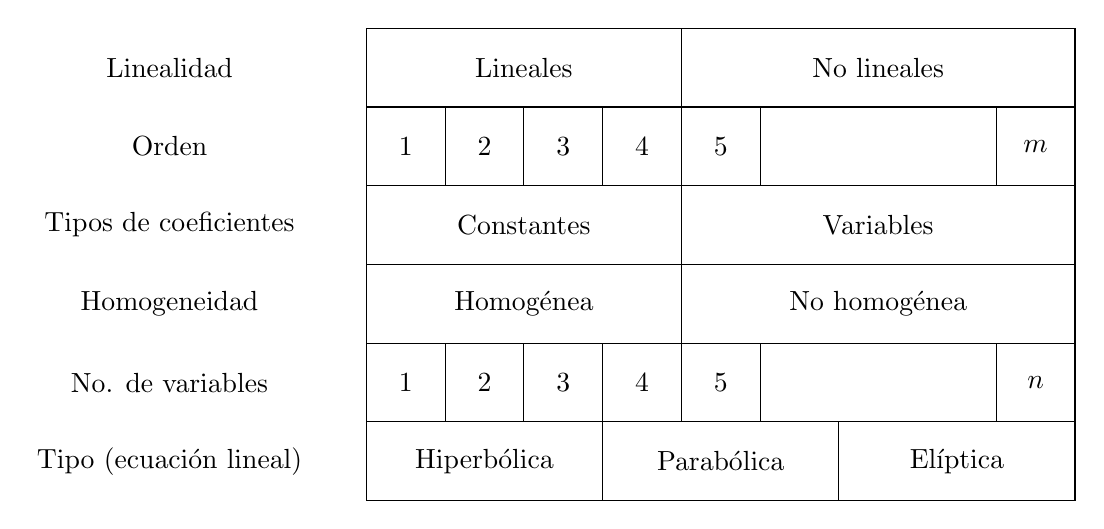
\begin{tikzpicture}

    \node at (-2.5, 0.5) {Tipo (ecuación lineal)};
    \draw (0, 0) rectangle (3, 1) node[pos=0.5] {Hiperbólica};
    \draw (3, 0) rectangle (6, 1) node[pos=0.5] {Parabólica};
    \draw (6, 0) rectangle (9, 1) node[pos=0.5] {Elíptica};

    \node at (-2.5, 1.5) {No. de variables};
    \draw (0, 1) rectangle (1, 2) node[pos=0.5] {$1$};
    \draw (1, 1) rectangle (2, 2) node[pos=0.5] {$2$};
    \draw (2, 1) rectangle (3, 2) node[pos=0.5] {$3$};
    \draw (3, 1) rectangle (4, 2) node[pos=0.5] {$4$};
    \draw (4, 1) rectangle (5, 2) node[pos=0.5] {$5$};
    \draw (5, 1) rectangle (8, 2);
    \draw (8, 1) rectangle (9, 2) node[pos=0.5] {$n$};

    \node at (-2.5, 2.5) {Homogeneidad};
    \draw (0, 2) rectangle (4, 3) node[pos=0.5] {Homogénea};
    \draw (4, 2) rectangle (9, 3) node[pos=0.5] {No homogénea};

    \node at (-2.5, 3.5) {Tipos de coeficientes};
    \draw (0, 3) rectangle (4, 4) node[pos=0.5] {Constantes};
    \draw (4, 3) rectangle (9, 4) node[pos=0.5] {Variables};
    
    \node at (-2.5, 4.5) {Orden};
    \draw (0, 4) rectangle (1, 5) node[pos=0.5] {$1$};
    \draw (1, 4) rectangle (2, 5) node[pos=0.5] {$2$};
    \draw (2, 4) rectangle (3, 5) node[pos=0.5] {$3$};
    \draw (3, 4) rectangle (4, 5) node[pos=0.5] {$4$};
    \draw (4, 4) rectangle (5, 5) node[pos=0.5] {$5$};
    \draw (5, 4) rectangle (8, 5);
    \draw (8, 4) rectangle (9, 5) node[pos=0.5] {$m$};

    \node at (-2.5, 5.5) {Linealidad};
    \draw (0, 5) rectangle (4, 6) node[pos=0.5] {Lineales};
    \draw (4, 5) rectangle (9, 6) node[pos=0.5] {No lineales};

\end{tikzpicture}
\end{document}